\section{Results}


Figure~\ref{fig:benchmark-perf} and Table \ref{tab:tuned-benchmark} shows the test accuracies for each method with and without the SOT module on both datasets.

% Without SOT:
% TM: (91.3 + 81.7 + 89.8 + 85.3 + 90)/5 = 87.6
% SP: (69.1 + 55.2 + 61.5 + 65.4 + 64.3)/5 = 63.1
Models without the SOT module reach an average accuracy of 88\% on the \texttt{TM} dataset and 63\% on the \texttt{SP} dataset. These results generally show that the models are capable of learning from few samples, improving significantly over the random baseline of 20\% accuracy. Peak performances in this group are achieved by \texttt{B} on both datasets, with 91\% and 69\% accuracy, respectively. The results indicate that \texttt{SP} is more challenging than the \texttt{TM} dataset. 

% With SOT:
% TM: (86.4 + 89.8 + 90.9 + 93.5 + 91.6)/5 = 90.4
% SP: (56.7 + 70.9 + 67.2 + 68.4 + 66.6)/5 = 65.9
Models incorporating the SOT module exhibit enhanced accuracy, achieving 90\% and 66\% average accuracy on the \texttt{TM} and \texttt{SP} dataset. While \texttt{MN}, \texttt{PN}, \texttt{MAML}, and \texttt{B++} show improved performance on \texttt{SP} when using SOT, \texttt{B} experiences a decline. Notably, \texttt{MN} on \texttt{SP} demonstrates the most significant gain with SOT: from a lowest accuracy of 55\% to the highest at 71\%. The addition of the SOT module increases the peak accuracy by 1.8 percentage points on \texttt{SP} and 2.2 on \texttt{TM}.

\textbf{Hyperparameter Ablation.} Figure~\ref{fig:hparams-swissprot-grid} shows the pair-wise interactions between all tuned hyperparameters. We also add a column for the methods to study how they react to certain hyper-parameters. 

The plots indicate a clear trend across all methods regarding the SOT hype-parameters: We find that using $\delta = cosine$ as a distance metric and regularisation with $\gamma = 0.1$ consistently yields the best performance. 
Furthermore, we find that all methods generally prefer lower learning rates of $\lambda=0.001$, especially in combination with a larger hidden dimension in the layers of the backbone. Finally, the plot reveals that \texttt{MN}, \texttt{PN}, and \texttt{MAML} are more robust to the choice of hyperparameters, yielding higher mean accuracies across tuning runs, while  \texttt{B++} was found especially sensitive. Despite being the best performing method on \texttt{SP}, its mean accuracy is lower in the tuning runs.

\begin{figure}[h!]
    \centering
    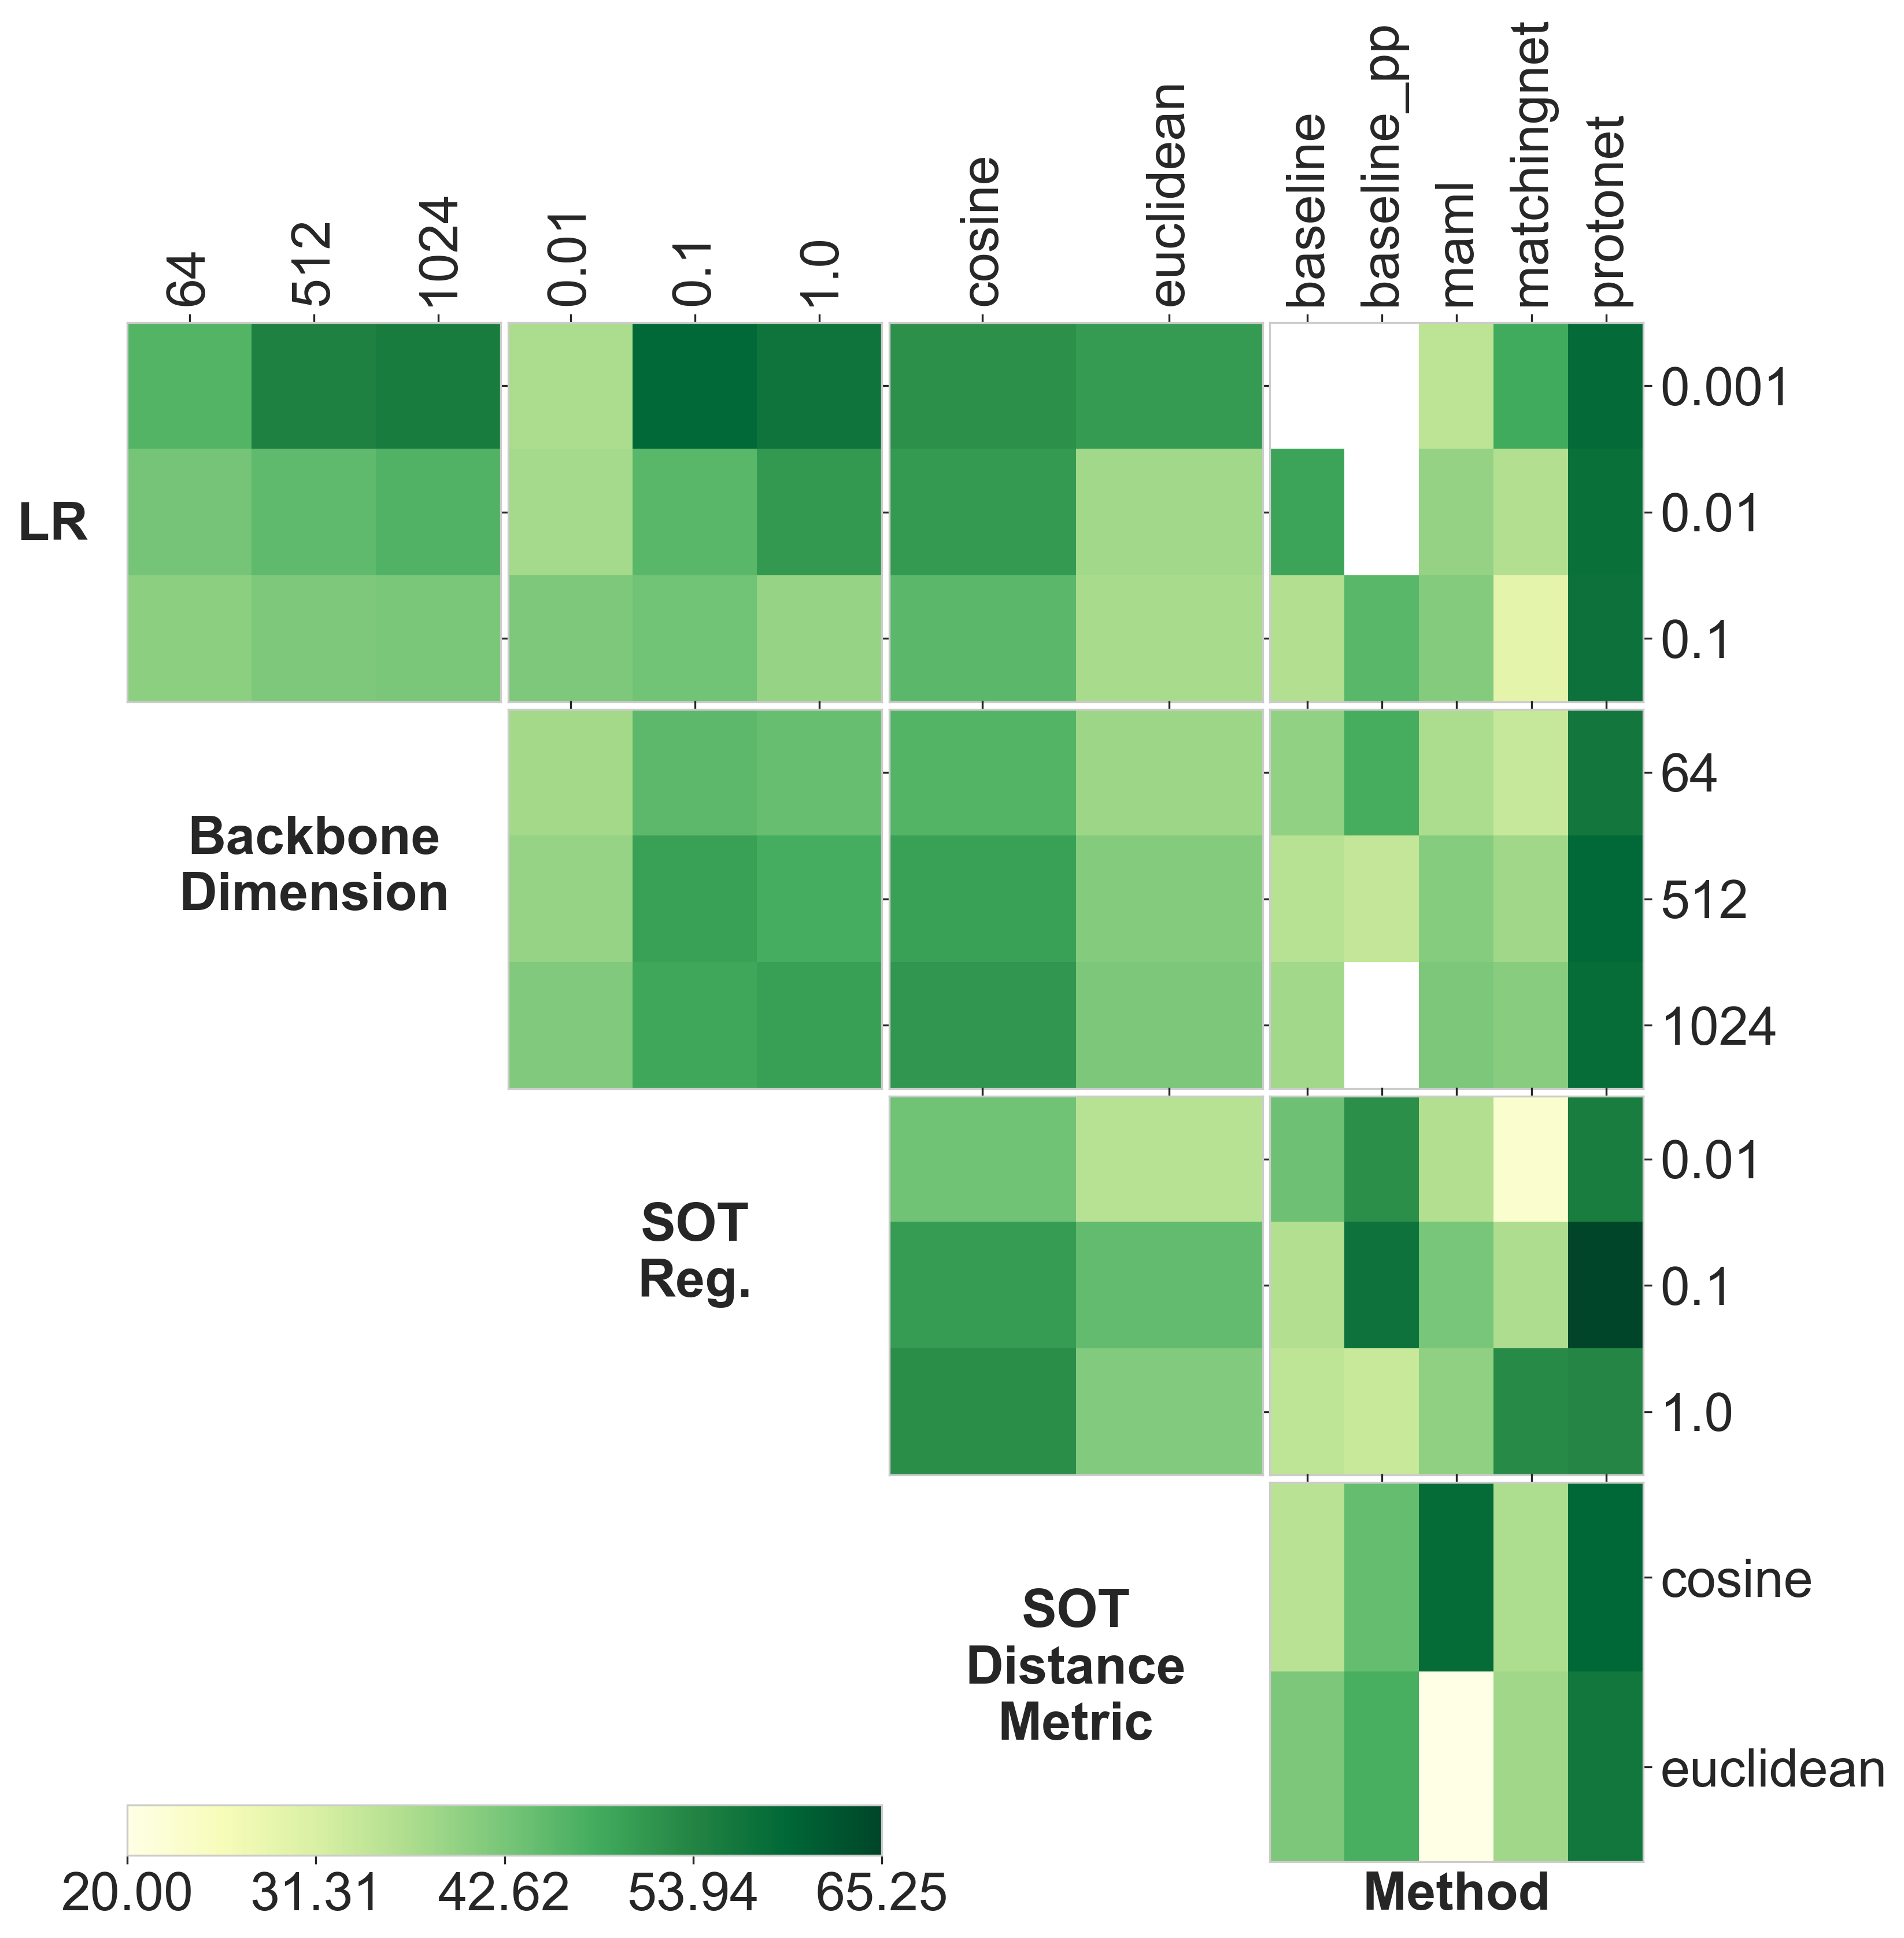
\includegraphics[width=1\columnwidth]{figures/hparams-interaction.png}
    \caption{\textbf{Hyperparameter Ablation.} Test accuracies on the \texttt{SP} dataset for all pairs of hyperparameter settings.}
    \label{fig:hparams-swissprot-grid}
\end{figure}

\begin{table}[ht]
\caption{
    \textbf{Benchmark Results.} Test accuracy of all methods on \texttt{TM} and \texttt{SP} in the 5-way-5-shot setting. We depict the average accuracy and the 95\% confidence interval both without (left) and with SOT (right) and the difference.
    \vspace{5pt}
}

\label{tab:tuned-benchmark}
\centering
\begin{tabular}{llllr}
\toprule
 &  & \multicolumn{2}{@{}c}{\textbf{Test Acc. (\%)}} & \\
 &  & w/o SOT & w/ SOT & Diff \\
\midrule
\multirow[c]{5}{*}{\texttt{TM}} & B & $90.7 \pm 0.7$ & $86.3 \pm 0.9$ & {\color{red} +4.8} \\
 & B++ & $81.9 \pm 0.9$ & $82.8 \pm 0.9$ &  {\color{teal} +1.1} \\
 & MAML & $\mathbf{92.8} \pm 0.5$ & $99.2 \pm 0.1$ & {\color{teal} +6.9} \\
 & MN & $84.6 \pm 0.8$ & $\mathbf{99.7} \pm 0.1$ &  {\color{teal} +17.9} \\
 & PN & $87.1 \pm 0.8$ & $98.6 \pm 0.2$ & {\color{teal} +13.2} \\
\midrule
\multirow[c]{5}{*}{\texttt{SP}} & B & $\mathbf{69.2} \pm 0.7$ & $55.7 \pm 0.8$ & {\color{red} -19.6} \\
 & B++ & $64.1 \pm 0.7$ & $64.6 \pm 0.7$ & {\color{teal} +0.8} \\
 & MAML & $68.7 \pm 0.7$ & $98.0 \pm 0.2$ & {\color{teal} +42.8} \\
 & MN & $68.2 \pm 0.8$ & $\mathbf{99.8} \pm 0.1$ & {\color{teal} +46.5} \\
 & PN & $63.5 \pm 0.7$ & $99.2 \pm 0.1$ & {\color{teal} +56.1} \\
\bottomrule
\end{tabular}
\end{table}

\textbf{Way-Shot Analysis.} Figure~\ref{fig:way-shot} illustrates \texttt{PN}'s way-shot analysis on the TM dataset, comparing scenarios with and without the SOT module. The left subplot depicts test accuracy versus the number of classes (ways), while the right subplot relates accuracy to the number of samples per class (shots). In both SOT and non-SOT contexts, a consistent trend emerges: accuracy diminishes linearly with more classes and grows with additional samples per class up to some limit. Notably, exceeding five samples per class yields no substantial accuracy gains. The model's performance with the SOT module is consistently inferior for higher numbers of classes and samples.

\begin{figure}[h!]
    \centering
    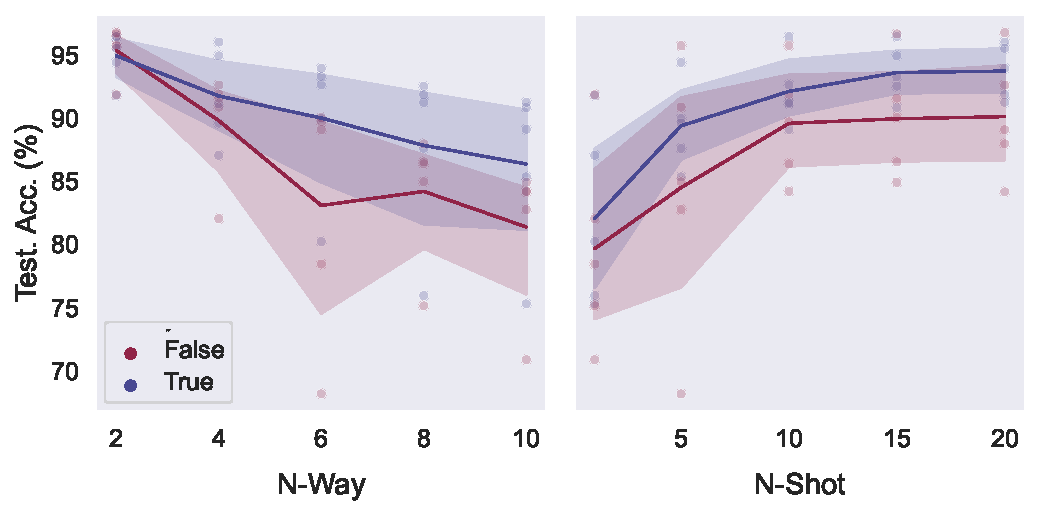
\includegraphics[width=1\columnwidth]{figures/way-shot.pdf}
    \caption{\textbf{Way-Shot Analysis.} Test accuracy of \texttt{PN} on the \texttt{TM} dataset with and without the SOT module in various 
    few-shot learning settings for fixed n-way (left) and n-shot (right). Individual points represent a single experiment. We show the regression line with a 95\% confidence interval.}
    \label{fig:way-shot}
\end{figure}
